\documentclass[11pt]{beamer}
\usefonttheme[onlymath]{serif}

\setbeamersize{text margin left=1.5em}
\setbeamersize{text margin right=1.5em}




\setbeamertemplate{frametitle}{%
  \vskip1ex
  \usebeamerfont{frametitle}%
  \insertframetitle\par %frame 에서 지정한 title 사용
  %\insertsubsectionhead\par        % subsection의 header를 사용
  \vskip1ex
  \hrule                             % 밑줄(선택)
}

\setbeamertemplate{blocks}[rounded][shadow=true] % 블록 테두리 둥글게

\setbeamertemplate{itemize item}{\usebeamerfont{itemize item}\textbullet}
\setbeamertemplate{itemize subitem}{\usebeamerfont{itemize subitem}\textbullet}
\setbeamertemplate{itemize subsubitem}{\usebeamerfont{itemize subsubitem}\textbullet}



%\setbeamerfont{itemize/enumerate subbody}{parent=itemize/enumerate body} % 
%\setbeamerfont{itemize/enumerate subbody}{size=\usebeamerfont{itemize/enumerate body}\size}

\makeatletter
% Taken from beamer.cls' default geometry settings
% http://mirrors.ctan.org/macros/latex/contrib/beamer/base/beamer.cls
\geometry{%
  papersize={\fpeval{\beamer@paperwidth*1.5}pt,\fpeval{\beamer@paperheight*1.5}pt},
  hmargin=\fpeval{0.5 * 1.5}cm,% 1cm
  vmargin=0cm,%
  head=\fpeval{0.5*1.5}cm,% 0.5cm
  headsep=0pt,%
  foot=\fpeval{0.5*1.5}cm% 0.5cm
}
\makeatother %from search keyword beamer size, get this search result -> https://tex.stackexchange.com/questions/586756/beamer-use-glyphs-from-smaller-font-size-but-enlarge


% Reference bibtex
% style = numeric, apa, authoryear-comp
\usepackage[backend=biber, style=authoryear-comp, natbib=true]{biblatex}
\addbibresource{../../../references.bib}



% 테마 선택 (선택 사항)
% \usetheme{Madrid} % 기본 테마, 다른 테마 사용 가능
% \font{serif}
\usepackage{amsfonts}
\usepackage{amssymb}
\usepackage[T1]{fontenc} % To use combination of textbf, textit
\usepackage[dvipsnames]{xcolor}   % can use more variant colors
%\usepackage{lmodern} %다른 폰트 사용: 문서의 서문에 추가하면 Computer Modern 폰트의 확장 버전인 Latin Modern 폰트를 사용할 수 있습니다. 이 폰트는 더 다양한 크기와 스타일을 지원하여 문제를 해결해 줄 수 있습니다.

% \setcounter{MaxMatrixCols}{20}

% (필요한 패키지들)
% \usepackage{amsthm}
\setbeamertemplate{theorems}[numbered]  % 정리, 정의 등에 번호를 달아줌

% \theoremstyle{plain} % insert bellow all blocks you want in italic
% \newtheorem{theorem}{Theorem}[section] % to number according to section
% 
% \theoremstyle{definition} % insert bellow all blocks you want in normal text
% \newtheorem{definition}{Definition}[section] % to number according to section
% \newtheorem*{idea}{Proof idea} % no numbered block

\newtheorem{proposition}[theorem]{Proposition}

\usepackage{tcolorbox}

% 필요할 경우 패키지 추가
\usepackage{graphicx} % 이미지 삽입을 위한 패키지
\usepackage{amsmath}   % 수식 사용
\usepackage{hyperref}  % 하이퍼링크 추가
\hypersetup{
  colorlinks=true,
  linkcolor=blue,
} % search keyword: beamer hyperref color -> https://tex.stackexchange.com/questions/13423/how-to-change-the-color-of-href-links-for-real
%search keyword: hyperref color -> https://www.overleaf.com/learn/latex/Hyperlinks
\usepackage{cleveref}
\usepackage{multicol}  % 여러 열 나누기
\usepackage{ulem} % 취소선 및줄 나누기
\usepackage{mathtools} % dcases
%\usepackage{xparse} % NewDocumentCommand
\usepackage[boxed, lined]{algorithm2e} % to use algorithm block



% \NewDocumentCommand{\DefThreeOp}{m}{%
%   % \csname #1\endcsname 라는 이름으로, 3개 인자를 받는 새 매크로를 정의
%   \expandafter\NewDocumentCommand\csname #1\endcsname{mmm}{%
%     \operatorname{#1}\!\bigl(##1,\,##2,\,##3\bigr)%
%   }%
% }

\newcommand{\mrm}[1]{\mathrm{#1}}
\newcommand{\mbb}[1]{\mathbb{#1}}
\newcommand{\mb}[1]{\mathbf{#1}}
\newcommand{\mc}[1]{\mathcal{#1}}
\newcommand{\tb}[1]{\textbf{#1}}
\newcommand{\ti}[1]{\textit{#1}}
\newcommand{\Pois}[1]{\operatorname{Pois}(#1)}

\newcommand{\myber}[1]{\operatorname{Bern}\!\left(#1\right)}
\newcommand{\Bin}[2]{\operatorname{Bin}\!\left(#1,#2\right)}
\newcommand{\NBin}[2]{\operatorname{NBin}\!\left(#1,#2\right)}
\newcommand{\mytoinf}[1]{#1 \rightarrow \infty}
\newcommand{\myexp}[1]{\exp{\left(#1\right)}}
\newcommand{\Unif}[2]{\operatorname{Unif}\!\left(#1, #2\right)}
\newcommand{\UnifOne}[1]{\operatorname{Unif}\!\left(#1\right)}
\newcommand{\mygeom}[1]{\operatorname{Geom}\!\left(#1\right)}
\newcommand{\Expo}[1]{\operatorname{Expo}\!\left(#1\right)}
\newcommand{\abs}[1]{\left\lvert #1 \right\rvert}
\newcommand{\floor}[1]{\left\lfloor #1 \right \rfloor}
\newcommand{\expec}[1]{\operatorname{E}\left[ #1 \right]}
\newcommand{\Var}[1]{\operatorname{Var}\left[#1\right]}
\newcommand{\myskew}[1]{\operatorname{Skew}\!\left[#1\right]}
\newcommand{\mykurt}[1]{\operatorname{Kurt}\!\left[#1\right]}
\newcommand{\mywei}[2]{\operatorname{Wei}\!\left(#1, #2\right)}
\newcommand{\Span}{\operatorname{Span}}
\newcommand{\Cov}[2]{\operatorname{Cov}\!\left(#1, #2\right)}
\newcommand{\intinfty}{\int_{-\infty}^\infty}
\newcommand{\Corr}[2]{\operatorname{Corr}\!\left(#1, #2\right)}
\newcommand{\Mult}[3]{\operatorname{Mult}_{#1}\!\left(#2, #3\right)}
\newcommand{\Beta}[2]{\operatorname{Beta}\!\left(#1, #2\right)}
\newcommand{\HGeom}[3]{\operatorname{HGeom}\!\left(#1, #2, #3\right)}
\newcommand{\NHGeom}[3]{\operatorname{NHGeom}\!\left(#1,#2, #3\right)}
\newcommand{\GammaDist}[2]{\operatorname{Gamma}\!\left(#1, #2\right)}
%\DefThreeOp{PHGeom}

\newcommand{\im}{\operatorname{im}}
\newcommand{\tr}{\operatorname{tr}}
\newcommand{\supp}{\operatorname{supp}}


% 발표 제목, 저자, 날짜 설정
\title{Off-Policy Deep Reinforcement Learning without Exploration (BCQ)}
\author{Gwanwoo Choi}
% \date{}

\begin{document}
% 표지 슬라이드

\begin{frame}
    \titlepage
\end{frame}

% \subsection{Domain Randomization}
% \begingroup
%     \setbeamertemplate{frametitle}{%
%     \vskip1ex
%     \usebeamerfont{frametitle}%
%     \insertframetitle\par        %  ← 원하는 대로 변경 가능
%     \vskip1ex
%     \hrule                             % 밑줄(선택)
%     }
%     \begin{frame}
%         \frametitle{Table of Contents}
%         \tableofcontents[currentsubsection]
%     \end{frame}
% \endgroup

% % 목차 

% \begin{frame}{Curriculum Learning}

% \end{frame}

\begin{frame}{Extrapolation Error}
    Extrapolation Error: an error in off-policy value learning which is introduced by \tb{the mismatch between the dataset and true state-action visitation of the current policy}.

    \begin{block}{Absent Data}
        If any state-action pair $(s,a)$ is unavailable, then error is introduced as some function of the amount of similar data and approximation error.
        This means that the estimate of $Q_\theta(s^\prime, \pi(s^\prime))$ may be arbitrary bad without sufficient data near $(s^\prime, \pi(s^\prime))$.
    \end{block}

    \begin{block}{Model Bias}
        In offline RL, the bellman operator $\mc{T}^\pi$ is approximated by sampling transitions $(s,a,r,s^\prime)$ from $\mc{B}$ to estimate the expectation over $s^\prime$.
        \[
            \mc{T}^\pi Q (s,a) \approx \mbb{E}_{\textcolor{red}{s^\prime \sim \mc{B}}}[r + \gamma Q(s^\prime, \pi(s^\prime))]
        \]
        Without infinite state-action visitation, this produces a biased estimate of the transition dynamics.
    \end{block}

    \begin{block}{Training Mismatch}
        Even with sufficient datat, batch $\mc{B}$ is fixed.
        In Deep Q-Learning in batch setting,
        \[
            \approx \frac{1}{\abs{\mc{B}}} \sum_{\textcolor{red}{(s,a,r,s^\prime) \in \mc{B}}} \abs{r + \gamma Q_{\theta^\prime}(s^\prime, \pi(s^\prime)) - Q_\theta (s,a)}^2
        \]
        If the distribution of batch mismatches with the distribution under the current policy, learned value function may poor estimate
    \end{block}
\end{frame}

\begin{frame}{Motivation}
    \begin{block}{Datasets for Experiment}    
        \begin{itemize}
            \item Final buffer : replay buffer gathered by training a DDPG agent over a million time steps.
            \item Concurrent : BCQ train concurrently, with the same replay buffer, as the behavioral DDPG policy.
            \item Imitation : dataset collected by an expert policy.
            \item Imperfect demonstration : With 30\% of dataset, action is randomly chosen. With remainings, expert policy selects actions randomly with adding high exploration noise $\mc{N}(0, 0.3)$
        \end{itemize}
    \end{block}

    % \begin{figure}
    %     \centering
    %     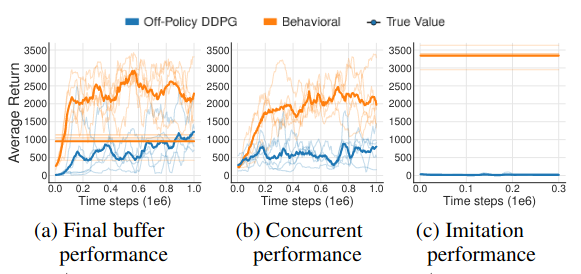
\includegraphics[width=0.65\textwidth]{Figure1Clipped.png}
    % \end{figure}
\end{frame}

\begin{frame}{Motivation}
    \begin{columns}
        \begin{column}{0.5\textwidth}
            \begin{figure}
                \centering
            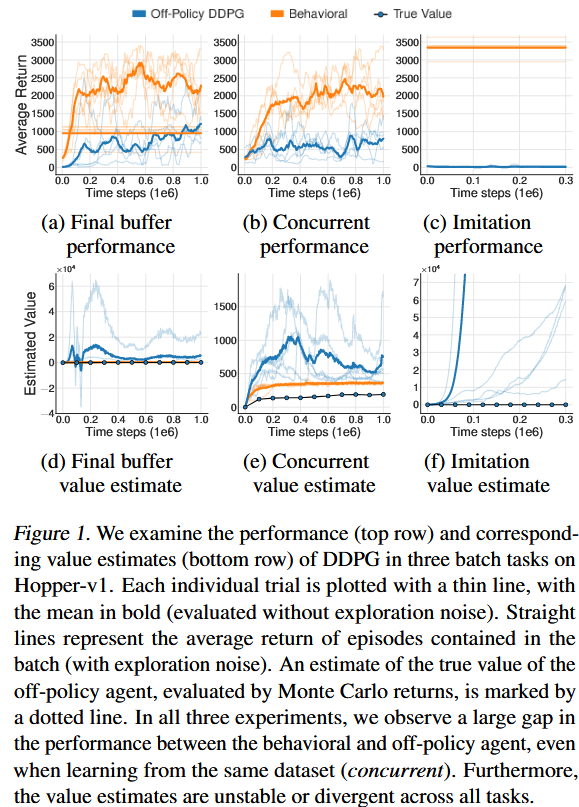
\includegraphics[width=0.9\textwidth]{figure1.png}
            \end{figure}
        \end{column}
        \begin{column}{0.5\textwidth}
            \begin{block}{Explanation of Figure 1}
                \begin{itemize}
                    \item Blue line is \tb{offline DDPG}, Orange line is \tb{behavioral DDPG}
                    \item Orange straight lines in above row represent the \tb{average return of episodes} contained in the batch
                    \item Dotted lines are estimates of the \tb{true value} of off-policy DDPG (this is evaluated by Monte Carlo returns)
                \end{itemize}
            \end{block}
            
            \begin{itemize}
                \item In each task, the offline agent \tb{performances significantly worse} than the behavioral agent.
                \item Even in the \tb{concurrent experiment}, where both agents are trained with the same dataset, there is \tb{a large gap} in performance in every single trial.
                \item In bottom row, offline agent has optimistic view for current state, whereas \tb{true value is much low}.
                % \item This result suggests that differences in the state distribution under the initial policies is enough for extrapolation error to drastically offset the performance of the off-policy agent.
            \end{itemize}
        \end{column}
    \end{columns}
\end{frame}

\begin{frame}{Batch-Constrained Reinforcement Learning}
    \begin{itemize}
        \item Batch Transition Probability: $p_{\mc{B}}(s^\prime|s,a) = \frac{N(s,a,s^\prime)}{\sum_{\tilde{S}}N(s,a,\tilde{s})}$
        \item Batch MDP $M_{\mc{B}}$ samples new state $s^\prime$ by $p_{\mc{B}}(s^\prime|s,a)$.
        
        
        \item Set $s_{\text{init}}$ as pseudo terminal state. If $\sum_{\tilde{s}} N(s,a, \tilde{s}) = 0$, then denote $p_{\mc{B}}(s_{\text{{init}}}|s,a) = 1$.
        
        Note that \underline{in batch constrained setting, for transition $(s,a,s_{\text{init}})$, $Q(s,a)$ will not update}.
        \item Batch-Constrained Policy $\pi \in \Pi_{\mc{B}}$ : $\forall (s,a), \mu_\pi(s)>0 \text{ and } \pi(a|s) > 0 \implies (s,a) \in \mc{B}$.
    \end{itemize}

    \begin{block}{Batch-Constrained Q-Learning (BCQL)}
        Batch-constrained Q-Learning follows the standard tabular Q-Learning update while constraining the possible actions with respect to the batch
        \[
            Q(s,a) \leftarrow (1-\alpha) Q(s,a) + \alpha \left(r + \gamma \max_{ \textcolor{red}{a^\prime \text{ s.t. }(s^\prime, a^\prime) \in \mc{B}}} Q(s^\prime, a^\prime) \right)
        \]
    \end{block}

    \vspace{0.5cm}
    Let denote $Q^\pi_{\mc{B}}$ be fixed point of batch-constrained Q-Learning and $Q^\pi$ be fixed point of Q-learning.
    \begin{block}{Theorem 4}
        \ti{Given a deterministic MDP and coherent batch $\mc{B}$, along with the Robbins-Monro stochastic convergence conditions on the learning rate $\alpha$ and standard sampling requirements on the batch $\mc{B}$, \ti{BCQL converges to $Q^{\pi}_\mc{B} (s,a)$ where $\pi^\ast(s) = \arg\max_{a \text{ s.t. }(s,a) \in \mc{B}} Q^\pi_{\mc{B}}(s,a)$ is the optimal batch-constrained policy}}

        \bigskip
        \ti{Proof.} BCQL learns optimal value for the MDP $M_{\mc{B}}$ by \hyperref[th:1]{theorem 1}.
        Also, by \hyperref[th:3]{theorem 3}, with sampling true transition dynamics of environments, BCQL also learns optimal value.
        If the MDP is deterministic, then by \hyperref[th:2]{theorem 2}, the optimal values obtained from theorem 1 and from theorem 3 are same.
        Therefore, if MDP is deterministic, then $\pi^\ast (s) = \arg \max_{a \text{ s.t. } (s,a) \in \mc{B}} Q^\pi_{\mc{B}}(s,a)$ is optimal policy.

    \end{block}

\end{frame}

\begin{frame}{Batch-Constrained Deep Reinforcement Learning}
    Theorem 4 tells us that with converged $Q^\pi_{\mc{B}}$, we can obtain \tb{optimal deterministic policy} as $\pi^\ast(s) = \arg \max_{a \text{ s.t. } (s,a) \in \mc{B}}Q^\pi_{\mc{B}}(s,a)$ in deterministic MDP.

    \vspace{1cm}
    So, BCQ approaches the notion of batch-constrained through a generative model for effectively considering $(s,a) \in \mc{B}$.
    \begin{itemize}
        \item For a given state, BCQ generates plausible candidate actions with high similarity to the batch.
        \item And then selects the highest valued action through a learned Q-Network.
    \end{itemize}

    Penalize Q value of rare, unseen states via modified version of TD3. (Critic update)
\end{frame}

\begin{frame}{Batch-Constrained Deep Reinforcement Learning}
    \tb{BCQ approaches the notion of batch-constrained through a generative model. (Policy update)}
    \begin{itemize}
        \item For a given state, BCQ generates plausible candidate actions with high similarity to the batch.
        \item And then selects the highest valued action through a learned Q-Network.
    \end{itemize}

    Penalize Q value of rare, unseen states via modified version of TD3. (Critic update)
    \bigskip

    \vfill

    \begin{enumerate}
        \item In ideal situation, we can learn \textcolor{magenta}{state-conditioned marginal likelihood $P^G_\mc{B}(a|s) \approx P_{\mc{B}}(a|s)$}.
        But it is difficult to learn $P^G_\mc{B}(a|s)$ in continuous state space and high-dimensional action space.
        $\implies$ We instead train a \tb{variational auto-endocer(VAE): $G_\omega (s)$}. This fucntion generates action $a$ by given state $s$.
        \item Generate $n$ actions $\{a_i\} \sim G_\omega (s)$.
        And define $\pi(s) \coloneqq \arg \max_{a_i} Q_\theta (s, a_i)$
        \item Increase diversity of selected action, with introducion of perturbation model, $\xi_\phi(s,a,\Phi)$, where $s,a$ is input and $\Phi$ is hyperparameter
        $\implies$ $\pi(s) \coloneqq \arg \max_{a_i + \xi_\phi(s,a_i, \Phi)} Q_\theta (s,a_i + \xi_\phi (s,a_i, \Phi)), \{a_i \sim G_\omega(s)\}_{i=1}^n$

    \end{enumerate}

    \begin{figure}
        \centering
        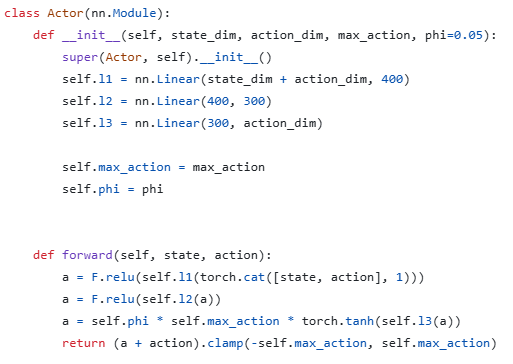
\includegraphics[width=0.5\textwidth]{Actor.png}
        \caption{Perturbation Model Code Snippet}
    \end{figure}
\end{frame}

\begin{frame}{Batch-Constrained Deep Reinforcement Learning}
    \tb{BCQ approaches the notion of batch-constrained through a generative model. (Policy update)}
    \begin{itemize}
        \item For a given state, BCQ generates plausible candidate actions with high similarity to the batch.
        \item And then selects the highest valued action through a learned Q-Network.
    \end{itemize}

    Penalize Q value of rare, unseen states via modified version of TD3. (Critic update)
    \bigskip

    \vfill

    Note that hyperparameters $n$ and $\Phi$ determine the ration between Imitation Learning and Reinforcement Learning.
    $\pi(s) \coloneqq \arg \max_{a_i + \xi_\phi(s,a_i, \Phi)} Q_\theta (s,a_i + \xi_\phi (s,a_i, \Phi)), \{a_i \sim G_\omega(s)\}_{i=1}^n$.
    \begin{itemize}
        \item If $n=1$ and $\Phi=0$, then the policy resembles behavior cloning
        \item If $n=\infty$ and $\Phi = a_{\text{max}} - a_{\text{min}}$, then the algorithm approaches Q-Learning, as the the policy begins to greedily maximize the value function over the entire action space.
    \end{itemize}
\end{frame}


\begin{frame}{Batch-Constrained Deep Reinforcement Learning}
    \tb{BCQ approaches the notion of batch-constrained through a generative model. (Policy update)}
    \begin{itemize}
        \item For a given state, BCQ generates plausible candidate actions with high similarity to the batch.
        \item And then selects the highest valued action through a learned Q-Network.
    \end{itemize}

    Penalize Q value of rare, unseen states via modified version of TD3. (Critic update)
    \bigskip

    \vfill

    The perturbation model $\xi_\phi$ can be trained to maximize $Q_\theta(s,a)$ through the DDPG style update by sampling $a \sim G_\omega (s)$
    \[
        \phi \leftarrow \arg\max_\phi \sum_{(s,a) \in \mc{B}} Q_\theta (s, a+ \xi_\phi (s,a, \Phi))
    \]
\end{frame}

\begin{frame}{Batch-Constrained Deep Reinforcement Learning}
    BCQ approaches the notion of batch-constrained through a generative model.
    \begin{itemize}
        \item For a given state, BCQ generates plausible candidate actions with high similarity to the batch.
        \item And then selects the highest valued action through a learned Q-Network.
    \end{itemize}

    \tb{Penalize Q value of rare, unseen states via modified version of TD3. (Critic update)}
    \bigskip

    \vfill

    To penalize uncertainty over future states, modify Clipped Double Q-Learning (TD3).
    The learning target used by both Q-Network is defined by
    \[
        y = r + \gamma \max_{a_i} \left[ \lambda \min_{j=1,2} Q_{\theta^\prime_j} (s^\prime,a_i) + (1-\lambda) \max_{j=1,2} Q_{\theta^\prime_j} (s^\prime, a_i)\right]
    \]
    \begin{itemize}
        \item A higher value of $\lambda$ places more weight on the minimum, while a lower value of $1 - \lambda$ places less weight on the maxmium.
        \item When a state $s$ is infrequent in the batch $\mc{B}$, it is likely that $Q_1$ and $Q_2$ will produce very different values.
        In this case, the minimum operator \tb{prevents overestimation} by selecting the lower (more conservative) value.
        \item Conversely, when a state $s$ is frequenty in the batch $\mc{B}$, $Q_1$ and $Q_2$ will likely have similar values.
        Here, the minimum operator has a \tb{lower effect}, and the penalty for overestimation is minimal.
    \end{itemize}
\end{frame}

\begin{frame}{Batch-Constrained Deep Reinforcement Learning}
    \begin{figure}
        \centering
        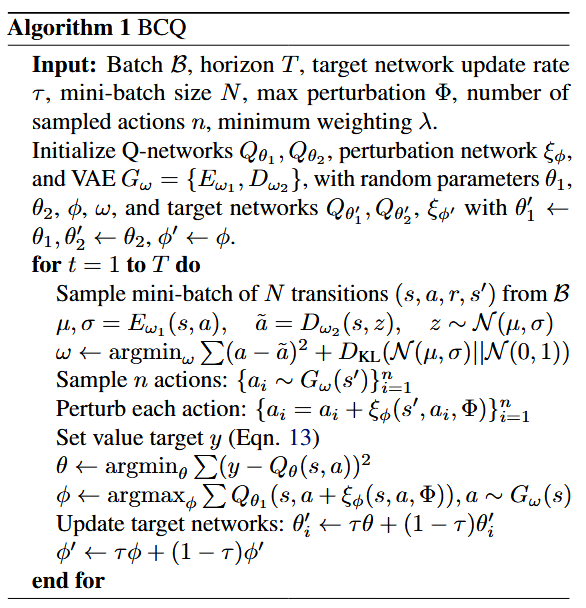
\includegraphics[width=0.5\textwidth]{algorithm.png}
    \end{figure}
    BCQ maintains four parametrized model: a generative model $G_\omega(s)$, a perturbation model $\xi_\phi (s,a)$, and two Q Networks $Q_{\theta_1}(s,a), Q_{\theta_2}(s,a)$.
\end{frame}


\begin{frame}{Experiments}
    \begin{columns}
        \begin{column}{0.45\textwidth}
            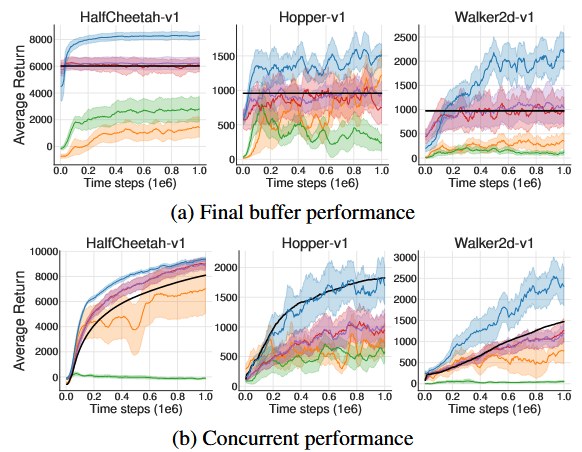
\includegraphics[width=1.0\textwidth]{figure2-1.png}
        \end{column}
        \begin{column}{0.45\textwidth}
            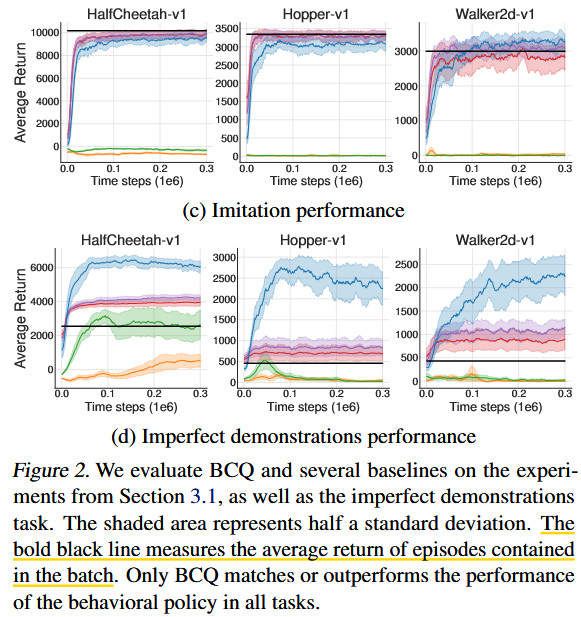
\includegraphics[width=1.0\textwidth]{figure2-2.png}
        \end{column}
    \end{columns}

    \smallskip
    \begin{itemize}
        \item \tb{BCQ is the only algorithm} which \tb{succeeds at all tasks}, matching or outperforming the behavioral policy in each instance, and outperforming all other agents.
        \item In the imperfect demonstrations task, we find that both deep reinforcement learning and imitation learning algorithms perform poorly. BCQ, however, is able to \tb{strongly outperforms the noisy demonstrator}, disentangling poor and expert actions.
        \item Compared to current deep reinforcement learning algorithms, which can requires millions of time steps, BCQ attains a high performance in remarkably \tb{few iterations}.
    \end{itemize}
\end{frame}

% \begin{frame}[t]{Experiments}
\begin{frame}{Experiments}
    \begin{figure}
        \centering
        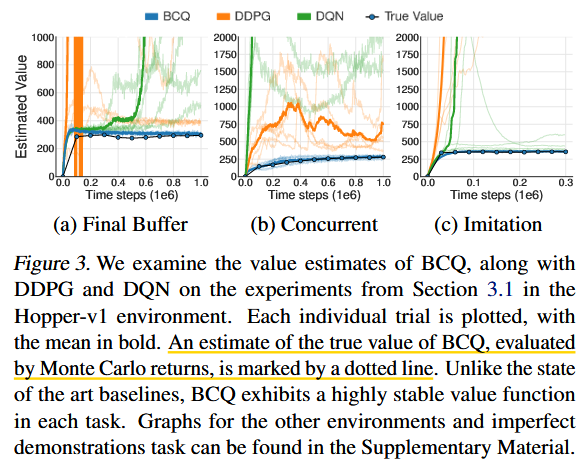
\includegraphics[width=0.5\textwidth]{figure3.png}
        \vfill
    \end{figure}

    \begin{itemize}
        \item BCQ exhibits a highly stable value function in the presence of off-policy samples, suggesting extrapolation error has been successfully mitigated through the batch-constraint.
    \end{itemize}
\end{frame}

\begin{frame}{Opinion}
    \begin{block}{Opinion}
        BCQ has restrict that it can only be utilized in \tb{deterministic MDP}. But in BEAR, there is no restrict about deterministic.
    \end{block}
\end{frame}

\begin{frame}{Proofs}
    \begin{itemize}
        \item Coherent Batch $M_{\mc{B}} : (s,a,s^\prime) \in \mc{B} \implies s^\prime \in \mc{B}$ 
        \item $\epsilon_{\text{MDP}}(s,a) \coloneqq Q^\pi (s,a) - Q^\pi_{\mc{B}}(s,a)$
        \item $\epsilon^\pi_{\text{MDP}} \coloneqq \sum_s \mu_\pi (s) \sum_a \pi(a|s) \abs{\epsilon_{\text{MDP}}(s,a)}$
        \item Optimal Batch-Constrained Policy $\pi^\ast \in \Pi_{\mc{B}} : \forall \pi \in \Pi_{\mc{B}}, \forall (s,a) \in \mc{B}, Q^{\pi^\ast}(s,a) \geq Q^\pi (s,a)$
        \item $p_{\mc{B}}(s^\prime|s,a) = \frac{N(s,a,s^\prime)}{\sum_{\tilde{s}}(s,a,\tilde{s})}$
        \item If $\sum_{\tilde{s}}(s,a,\tilde{s}) = 0$, then $p_{\mc{B}}(s_{\text{init}}|s,a)=1$, where $r(s_{\text{init}}, s, a)$ is initialized value of $Q(s,a)$
    \end{itemize}

    \begin{block}{Batch-Constrained Q-Learning (BCQL)}
        Batch-Constrained Q-Learning (BCQL) maintains a tabular value function $Q(s,a)$ for each possible state-action pair $(s,a)$.
        A transition tuple $(s,a,r,s^\prime)$ is sampled from the batch $\mc{B}$ with uniform probability and the following update rule  is applied, with learning rate $\alpha$:
        \[
            Q(s,a) \leftarrow (1- \alpha) Q(s,a) + \alpha (r + \gamma \max_{a^\prime \text{ s.t. } (s^\prime, a^\prime) \in \mc{B}} Q(s^\prime, a^\prime))
        \]
    \end{block}

    \begin{block}{Theorem 1} \label{th:1}
        Performing Q-Learning by sampling from a batch $\mc{B}$ converges to the optimal value function under the MDP $M_{\mc{B}}$
    \end{block}
\end{frame}

\begin{frame}{Proofs}
    \begin{block}{Remark 1}
        For any policy $\pi$ and state-action pair $(s,a)$, the error term $\epsilon_{\text{MDP}}(s,a)$ satisfies the following Bellman-like equation
        \[
        \begin{aligned}
            \epsilon_{\text{MDP}}(s,a) &= \sum_{s^\prime} (p_M(s^\prime|s,a) - p_{\mc{B}}(s^\prime|s,a)) \left(r(s,a,s^\prime)+\gamma \sum_{a^\prime}\pi(a^\prime | s^\prime) Q^\pi_{\mc{B}}(s^\prime, a^\prime) \right) \\
            &+ p_M(s^\prime |s,a) \gamma \sum_{a^\prime} \pi(a^\prime |s^\prime) \epsilon_{\text{MDP}}(s^\prime, a^\prime)
        \end{aligned}
        \]

        \smallskip
        Proof
        \[
        \begin{aligned}
            \epsilon_{\text{MDP}}(s,a) &= Q^{\pi}(s,a) - Q^\pi_{\mc{B}}(s,a) \\
            =& \sum_{s^\prime} p_M(s^\prime|s,a) \left(r(s,a,s^\prime) + \gamma \sum_{a^\prime} \pi(a^\prime|s^\prime) Q^\pi(s^\prime, a^\prime)\right) \\
            &- \sum_{s^\prime}p_{\mc{B}}(s^\prime|s,a) \left(r(s,a,s^\prime) + \gamma \sum_{a^\prime} \pi(a^\prime|s^\prime) Q^\pi_{\mc{B}}(s^\prime, a^\prime)\right) \\
            =&\sum_{s^\prime} \Big[(p_M(s^\prime|s,a) - p_{\mc{B}}(s^\prime|s,a))r(s,a,s^\prime) + p_M(s^\prime|s,a) \gamma \sum_{a^\prime} \pi(a^\prime|s^\prime) (Q^\pi_{\mc{B}}+\epsilon_{\text{MDP}}(s^\prime,a^\prime))\\
            & - p_{\mc{B}}(s^\prime|s,a) \gamma \sum_{a^\prime} \pi(a^\prime|s^\prime) Q^\pi_{\mc{B}}(s^\prime, a^\prime) \Big] \\
            \label{eq:remark1}
            =& \sum_{s^\prime} \Big[(p_M(s^\prime|s,a) - p_{\mc{B}}(s^\prime|s,a))\left(r(s,a,s^\prime) + \gamma \sum_{a^\prime}\pi(a^\prime|s^\prime) Q^\pi_{\mc{B}}\right) \\
            &+ p_M(s^\prime|s,a) \gamma \sum_{a^\prime} \pi(a^\prime|s^\prime)\epsilon_{\text{MDP}}(s^\prime,a^\prime) \Big]
        \end{aligned}
        \]
    \end{block}
\end{frame}

\begin{frame}{Proofs}
    \begin{block}{Lemma 1}
        For all reward functions, $\epsilon^\pi_{\text{MDP}} =0 \iff p_{\mc{B}}(s^\prime|s,a) = p_M(s^\prime|s,a)$ for all $s^\prime \in \mc{S}$ and $(s,a)$ such that $\mu_\pi (s) > 0$ and $\pi(a|s) > 0$.

        \smallskip
        Proof

        ($\implies$) From \hyperlink{eq:remark1}{remark 1}, $\epsilon_{\text{MDP}}(s,a) =0 \implies $
        \[
        0 = \sum_{s^\prime} (p_M(s^\prime|s,a) - p_{\mc{B}}(s^\prime|s,a)) \left(r(s,a,s^\prime) + \gamma \sum_{a^\prime}\pi(a^\prime|s^\prime) Q^\pi_{\mc{B}}(s^\prime,a^\prime)\right)
        \]
        $\implies p_M (s^\prime|s,a) = p_{\mc{B}}(s^\prime|s,a)$.

        ($\impliedby$) We can expand $\epsilon_{\text{MDP}}(s,a)$ terms recursively.
        Since $p_M(s^\prime|s,a) - p_{\mc{B}}(s^\prime|s,a) = 0$, $\epsilon_{\text{MDP}}(s,a) = 0 + \gamma 0 + \gamma^2 0 + \cdots  = 0$.
    \end{block}
    \begin{block}{Theorem 2} \label{th:2}
        \ti{For a deterministic MDP and all reward functions, $\epsilon^\pi_{\text{MDP}}=0 \iff$ the policy $\pi$ is batch-constrained.
        Furthermore, if $\mc{B}$ is coherent, then such a policy must exist if the start state $s_0 \in \mc{B}$.
        }

        Proof. In deterministic MDP, $P_M(s^\prime |s,a) = p_{\mc{B}}(s^\prime|s,a) =1$. So, the policy $\pi$ is batch-constrained. (First part)
        Since the MDP is deterministic and $\mc{B}$ is coherent, when starting from $s_0$, there must be able to follow at least one trajectory until termination. (Second part)
    \end{block}
    \begin{block}{Theorem 3} \label{th:3}
        \ti{Given the Robbins-Monro stochastic convergence conditions on the learning rate $\alpha$, and standard sampling requirements from the environment, BCQL converges to the optimal value function $Q^\ast$}.

        Proof. Nothing the batch-constraint is non-restrictive with a batch which contains all possible transitions.
    \end{block}
\end{frame}


\end{document}